\chapter{Odczytywanie losowego wyniku z kości}\label{ch:odczytywanie-losowego-wyniku-z-kosci}

Kolejnym krokiem przetwarzania jest odczyt wylosowanej wartości z kości,
jednak jak pokazano na rysunku~\ref{fig:schemat_workflow}
najpierw zdjęcie musi zostać poddane odpowiedniemu przetwarzaniu, które zostało opisane w tym rozdziale.

Rysunek~\ref{fig:schemat_workflow} w formie tekstowej
\begin{verbatim}
    Maszyna (robot) wykonuje rzut kością
    Kamera umieszczona w jego górnej części robi zdjęcie
    Zdjęcie to jest przekazywane do algorytmu wykonującego preprocessing
    Następnie, wyuczony przez nas model SI odczytuje wyrzucony na kości wynik i zwraca cyfrę
    Cyfra jest przekazywana na wyjście
\end{verbatim}

\begin{figure}[H]
    \centering
    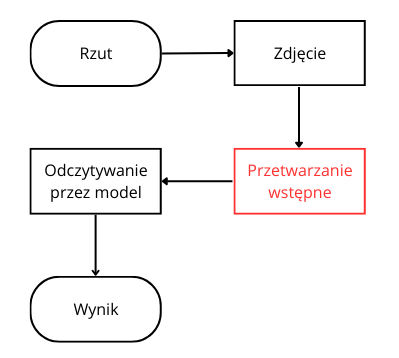
\includegraphics[width=0.5\linewidth]{chapters/04-czytanie/figures/schemat}
    \caption{Ten schemat jest do zmiany na ładniejszy, ale ja nie umiem rysować więc jest taki "na teraz"}
    \label{fig:schemat_workflow}
\end{figure}

\section{Przetwarzanie wstępne obrazów}\label{sec:preprocessing}

W niniejszym rozdziale omówiono proces przetwarzania wstępnego obrazów kości,
który przekształca dane pochodzące z fizycznego komponentu naszej maszyny (zdjęcia kości) na dane wejściowe dla modelu sztucznej inteligencji.
Przez dane wejściowe dla modelu SI rozumie się tutaj odpowiednio sformatowane obrazy, a więc takie w skali szarości,
o rozmiarach 64x64 piksele, zawierające jedynie kość wyciętą ze zdjęcia całego bębna maszyny.

\subsection{Algorytm}\label{subsec:algorytm}

Przetwarzanie obrazów składa się z kilku etapów, które dokładnie opisano poniżej, a przepływ pracy prezentuje się tak: \\
1. Wczytanie obrazu wejściowego \\
2. Odnalezienie kości za pomocą maski na komponencie nasycenia \\
3. Stworzenie i wycięcie ramki ograniczającej (ang. bounding box) wokół maski \\
4. Przeskalowanie do odpowiedniego rozmiaru \\
5. Konwersja do skali szarości \\
6. Zapisanie gotowego obrazu \\


Na rysunku~\ref{fig:preproc_steps} przedstawiono przykładowe zdjęcie surowe~\ref{fig:step1}
oraz kolejne etapy przetwarzania, aż do finalnego etapu~\ref{fig:step5}.

\begin{figure}[H]
    \centering
    \begin{subfigure}[t]{0.32\linewidth}
        \centering
        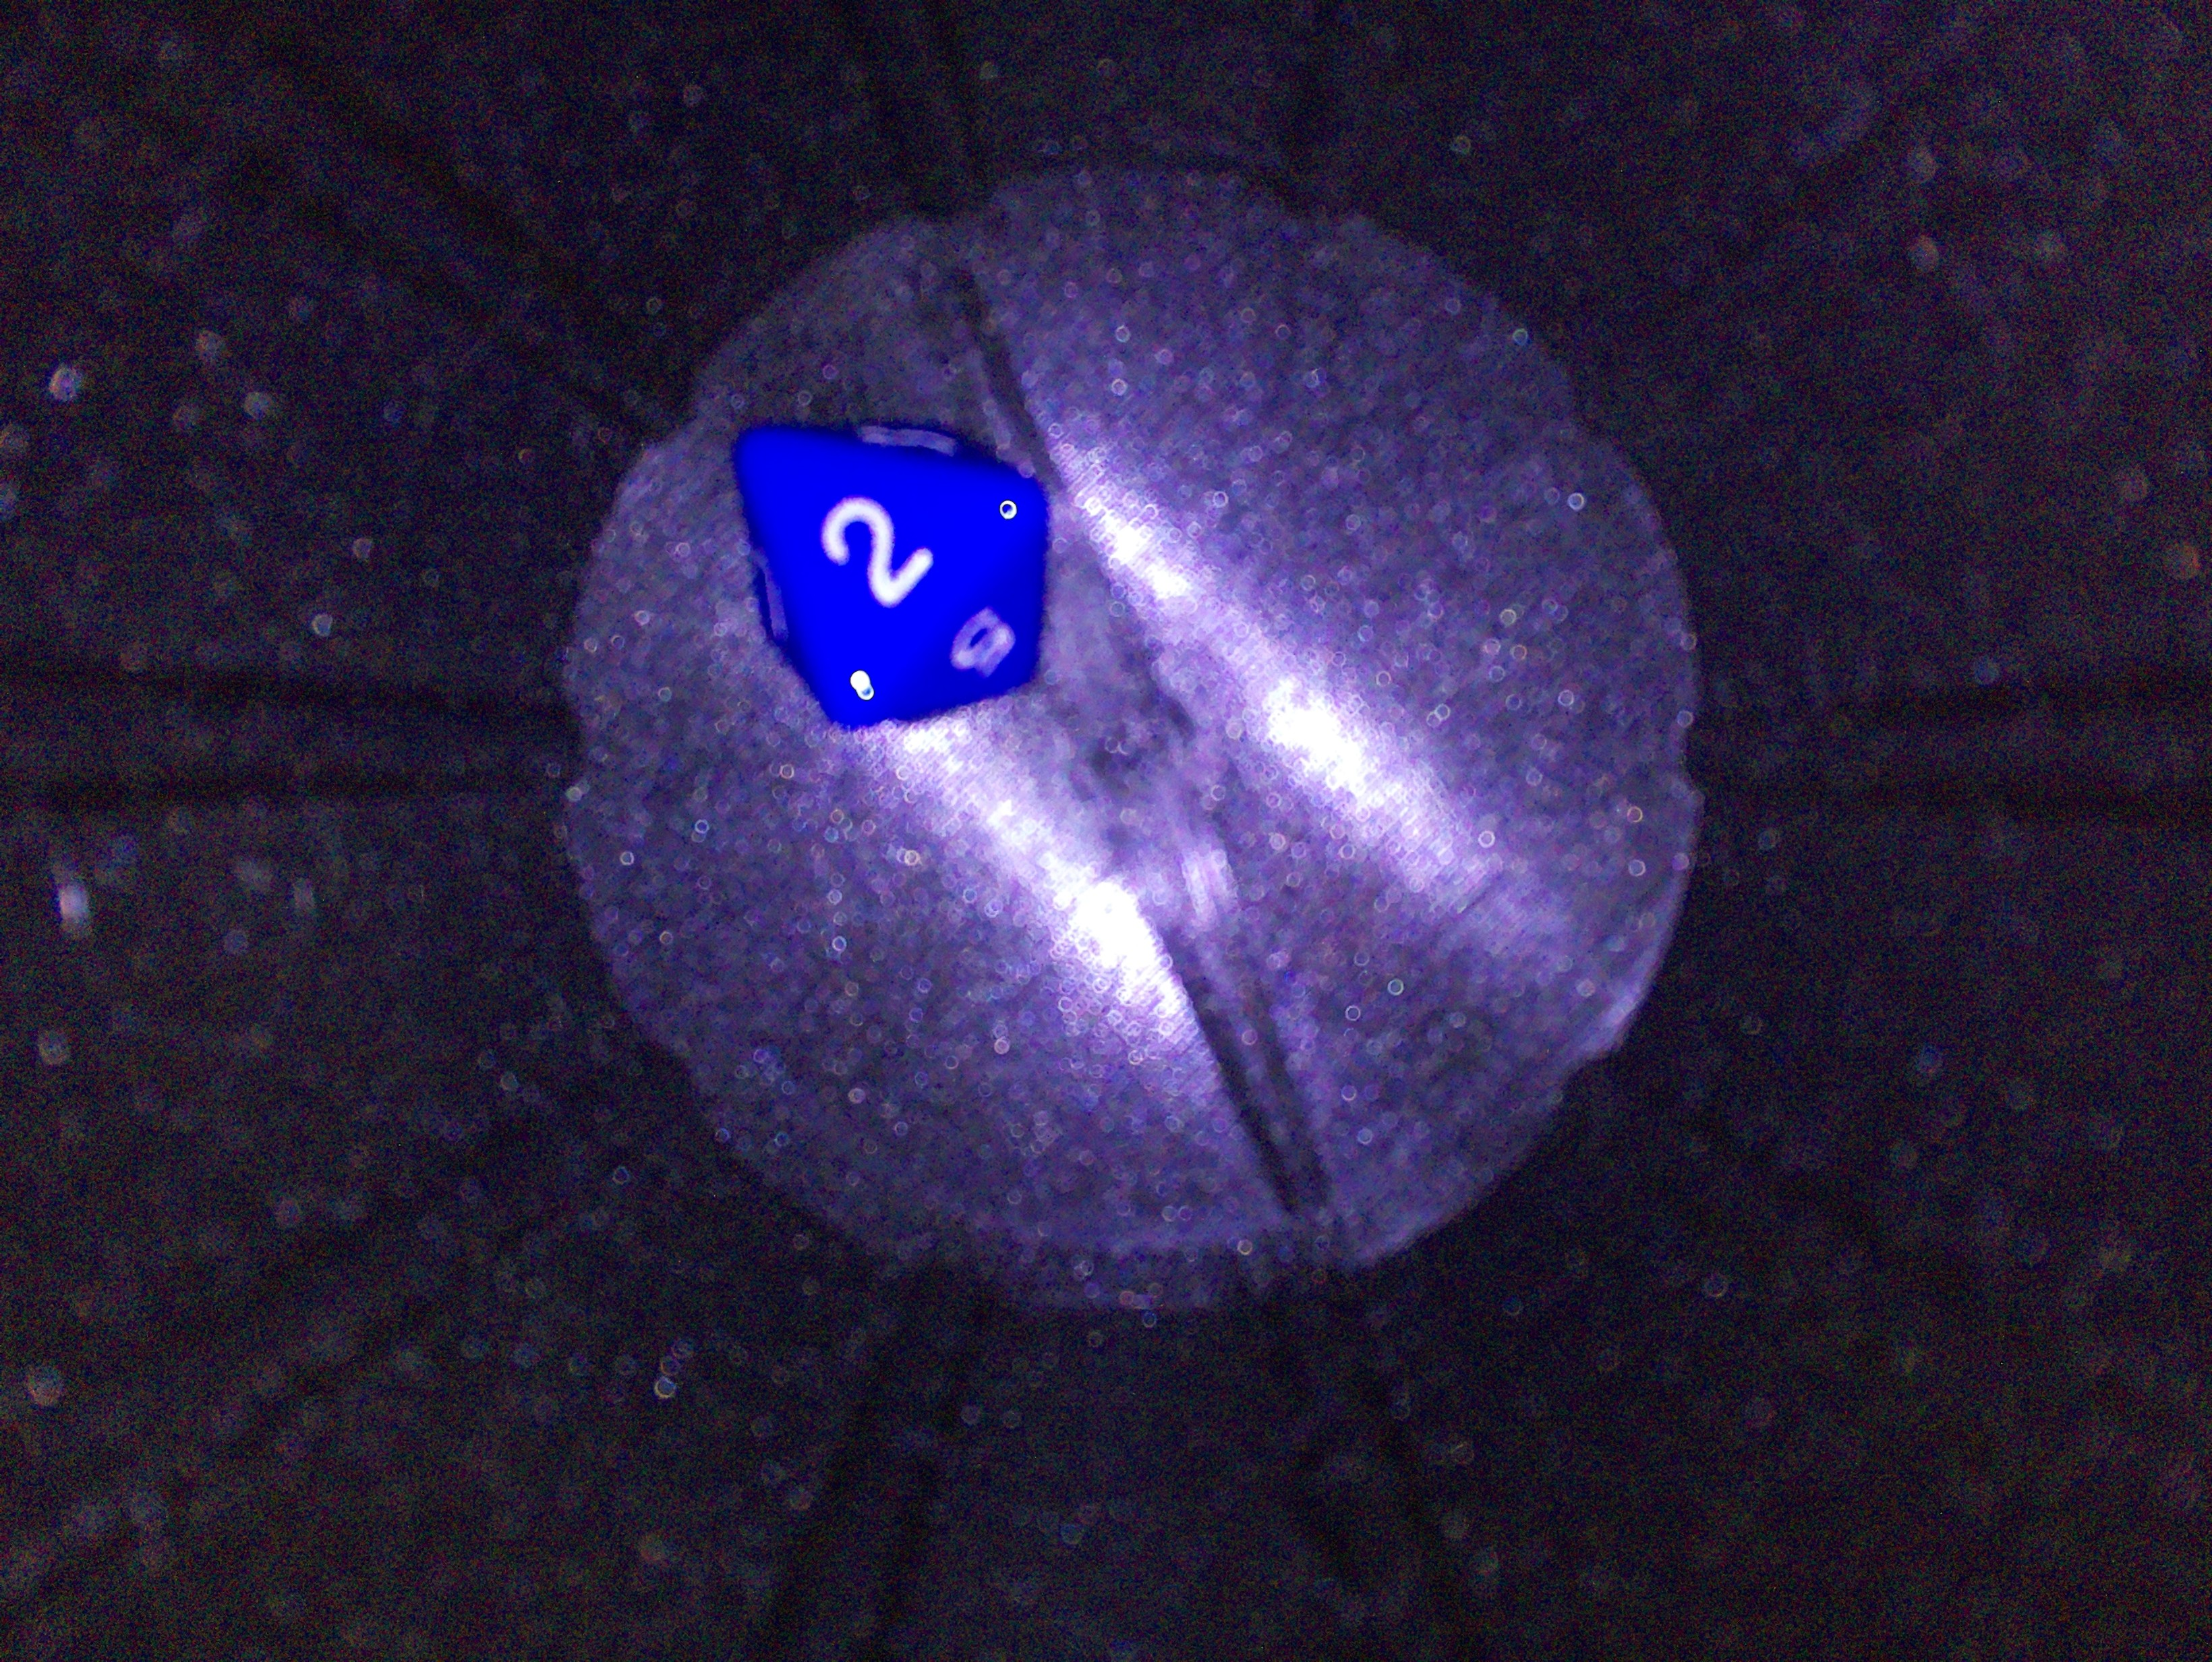
\includegraphics[height=4cm]{chapters/04-czytanie/figures/2_1}
        \caption{Etap 1: Surowe zdjęcie.}
        \label{fig:step1}
    \end{subfigure}
    \hfill
    \begin{subfigure}[t]{0.32\linewidth}
        \centering
        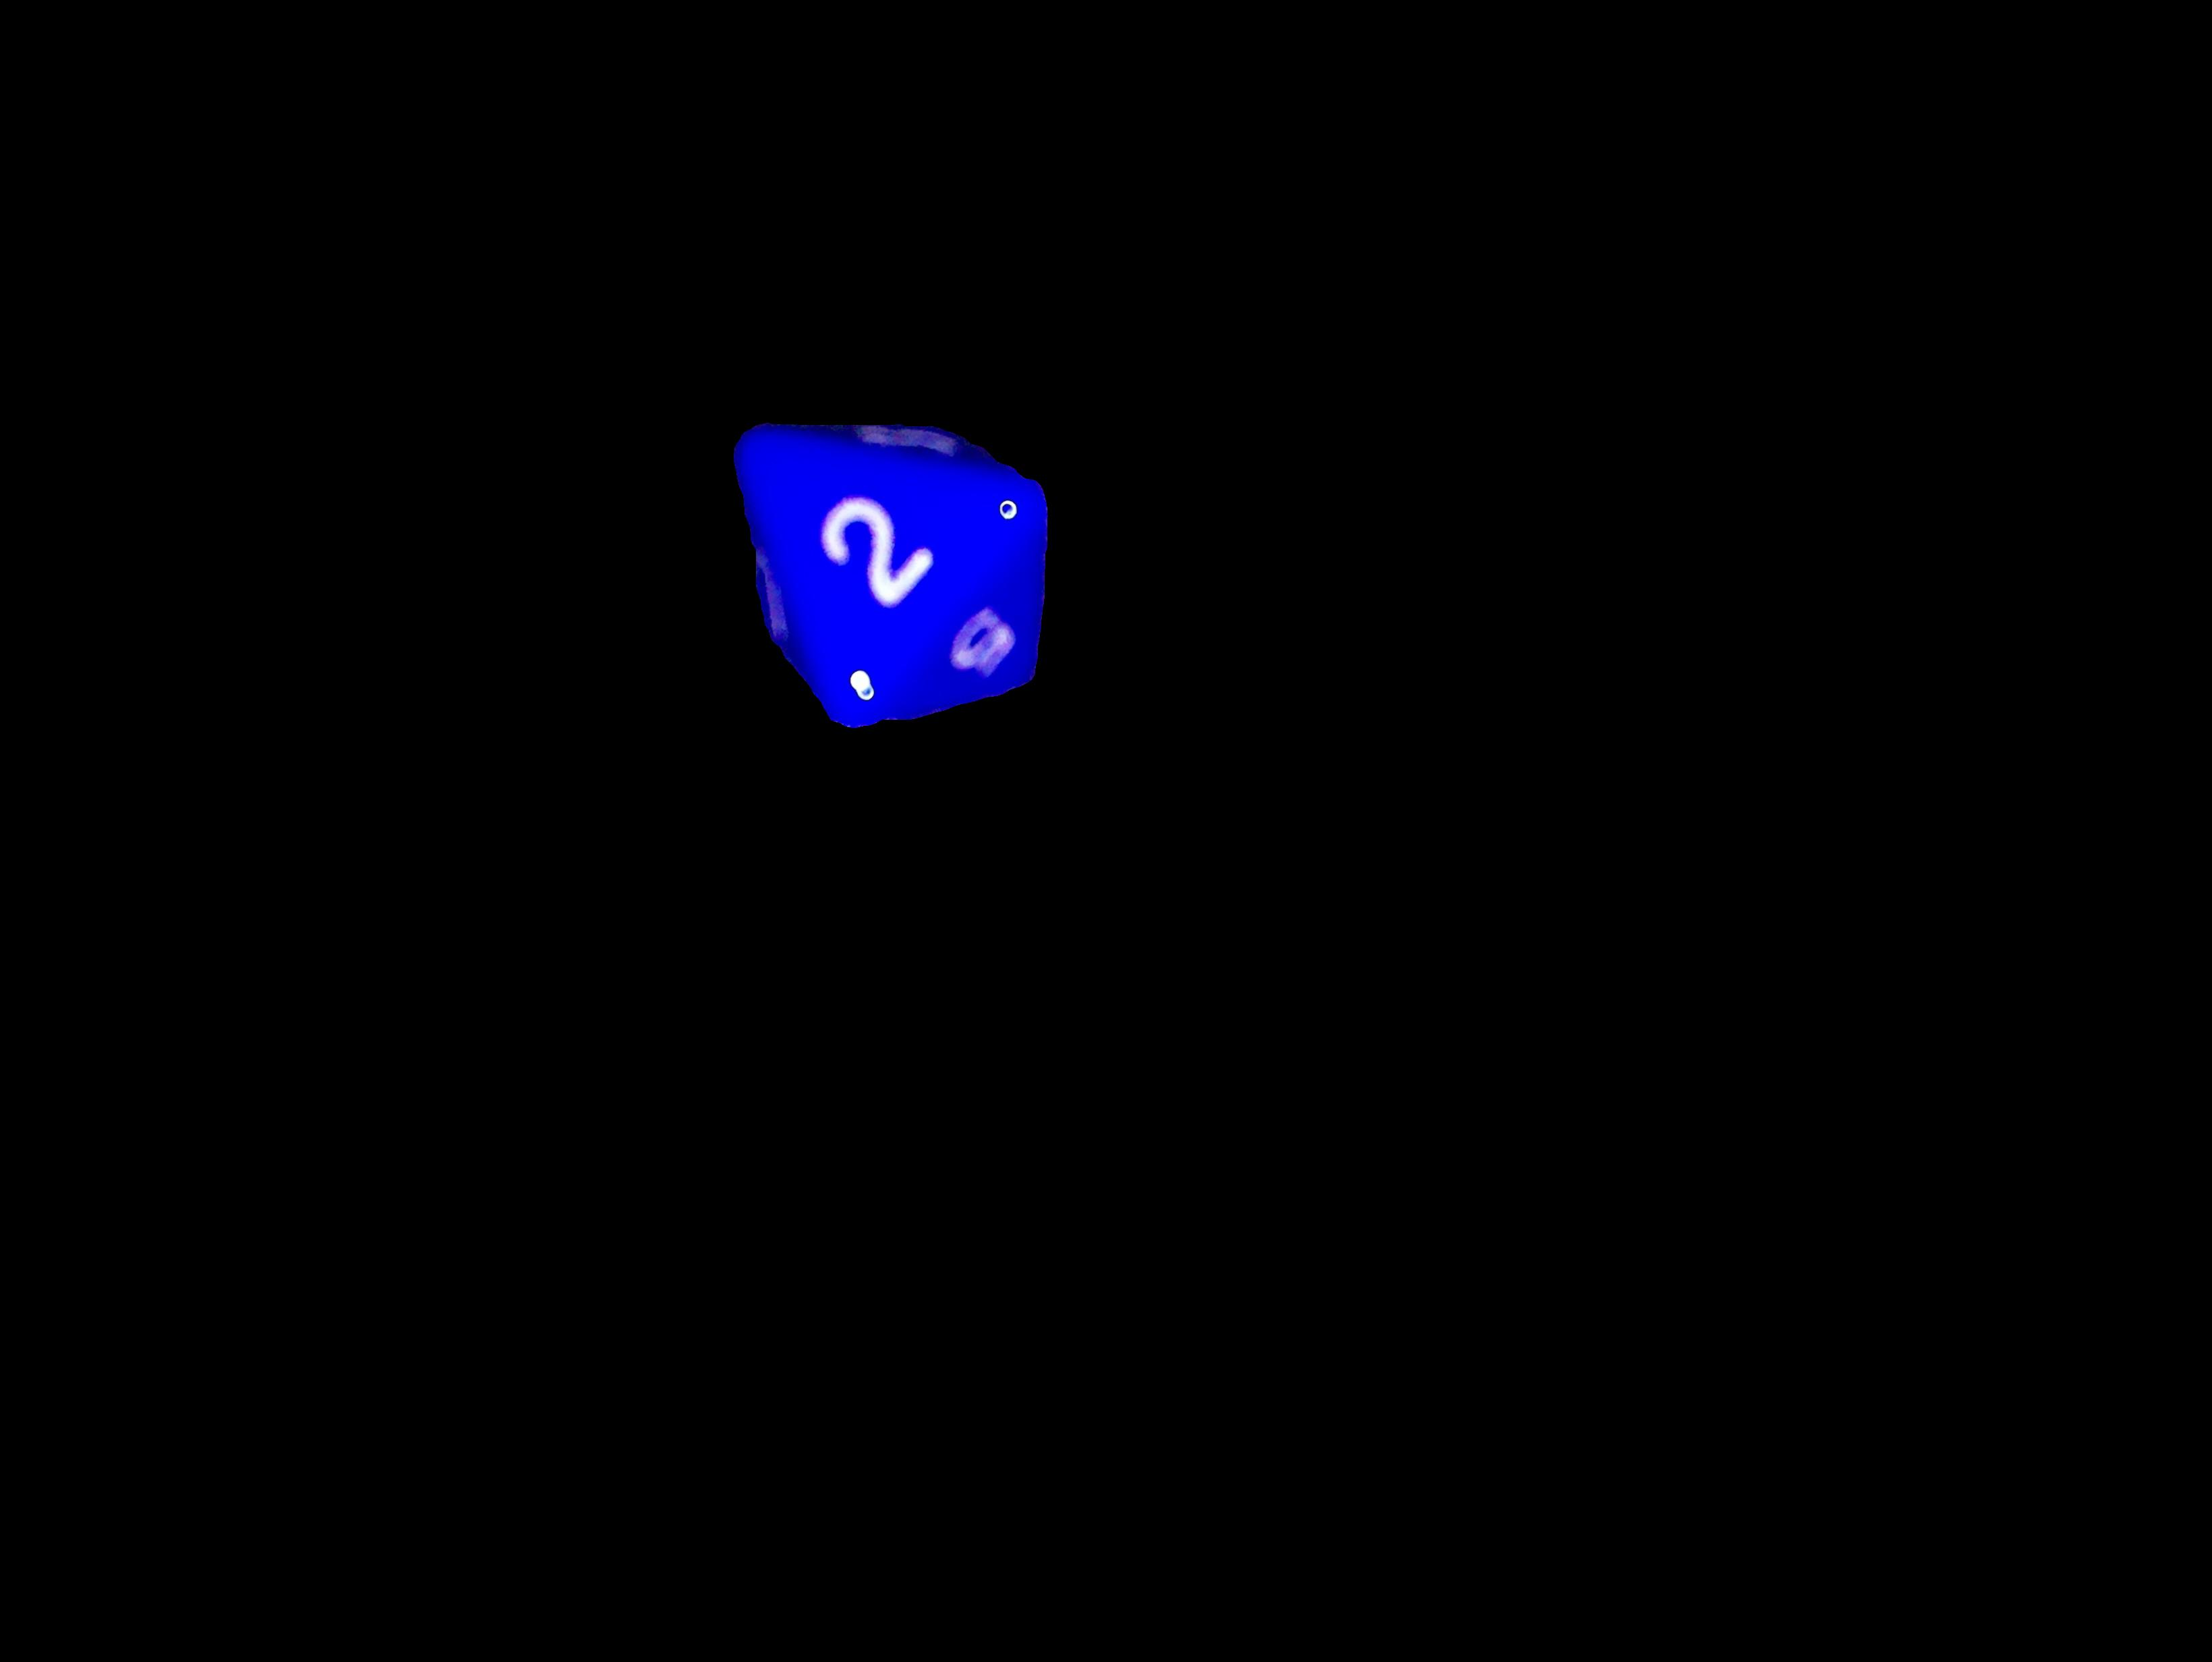
\includegraphics[height=4cm]{chapters/04-czytanie/figures/2_2}
        \caption{Etap 2: Nałożenie maski}
        \label{fig:step2}
    \end{subfigure}
    \hfill
    \begin{subfigure}[t]{0.32\linewidth}
        \centering
        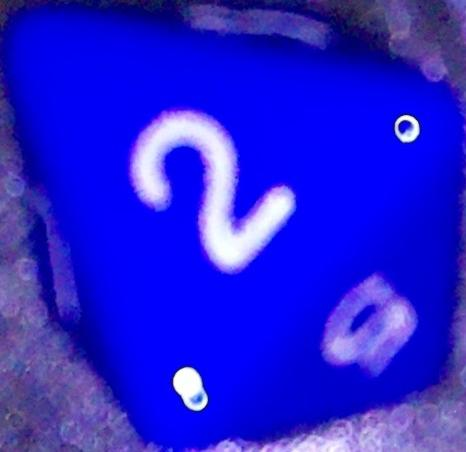
\includegraphics[height=4cm]{chapters/04-czytanie/figures/2_3}
        \caption{Etap 3: Wycięcie obszaru zainteresowania}
        \label{fig:step3}
    \end{subfigure}

    \vspace{0.5cm}

    \begin{subfigure}[t]{0.45\linewidth}
        \centering
        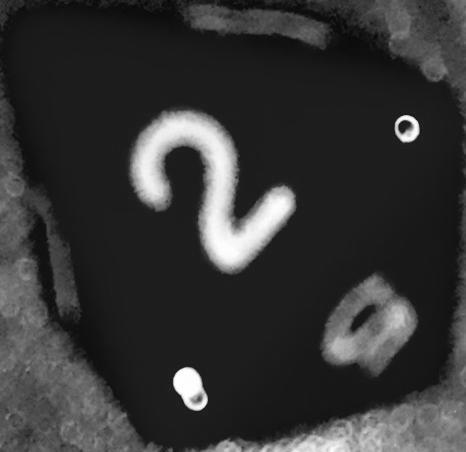
\includegraphics[height=4cm]{chapters/04-czytanie/figures/2_4}
        \caption{Etap 4: Skala szarości}
        \label{fig:step4}
    \end{subfigure}
    \hfill
    \begin{subfigure}[t]{0.45\linewidth}
        \centering
        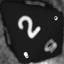
\includegraphics[height=4cm]{chapters/04-czytanie/figures/2_5}
        \caption{Etap 5: Wynik końcowy.}
        \label{fig:step5}
    \end{subfigure}

    \caption{Kolejne etapy przetwarzania obrazu. Wszystkie obrazy mają równą wysokość.}
    \label{fig:preproc_steps}
\end{figure}


Przedstawiony algorytm został zaimplementowany w języku Python, a jego zadaniem jest identyfikacja,
wycięcie i przeskalowanie obszarów zawierających obiekty zainteresowania na zdjęciach.

Zdjęcia w formacie JPEG są wczytywane za pomocą modułu Pillow~\cite{pillow_docs},
który umożliwia konwersję obrazów do przestrzeni barw RGB, zapewniając jednolitość formatów danych wejściowych.
Następnie obrazy są przekształcane do przestrzeni barw HSV,
co pozwala oddzielić komponenty odpowiadające za barwę (H), nasycenie (S) oraz jasność (V).

Komponent nasycenia (S) jest wygładzany za pomocą filtru Gaussa~\cite{gaussian_filter},
również dostępnego w ramach tego samego modułu,
co redukuje szumy i pozwala na bardziej precyzyjną analizę.
Wykorzystano parametry filtru z maską o wymiarach $5 \times 5$ pikseli oraz odchyleniem standardowym równym 1.
Takie ustawienia zapewniają balans między wygładzeniem a zachowaniem szczegółów obrazu.

Na podstawie wygładzonego komponentu nasycenia za pomocą progowania tworzona jest maska binarna,
która identyfikuje obszary o wysokim nasyceniu, odpowiadające obiektom zainteresowania (np. kości).
Próg został dobrany eksperymentalnie, kończąc na wartości 224,
tak aby w kontrolowanym środowisku (opisanym w poprzednim rozdziale) maska obejmowała obszar zainteresowania,
ale nie obejmowała tła (np. czarnego kubka).
Korzysta to z faktu, że kubek wykonany jest z materiału o niskim nasyceniu,
a używana kość ma jednolity, jasny kolor, a więc i wysokie nasycenie.

W celu usunięcia niewielkich luk w masce binarnej stosowana jest operacja zamknięcia morfologicznego~\cite{morphological_closure}.
Operacja ta ujednolica maskę, co jest szczególnie istotne w przypadku obiektów o niejednorodnej strukturze nasycenia,
gdzie maska mogłaby zawierać rozłączne fragmenty obiektu.

Po zastosowaniu zamknięcia morfologicznego maska jest analizowana w celu
zlokalizowania największego konturu obejmującego obszar zainteresowania.
W tym celu wykorzystano funkcje biblioteki OpenCV~\cite{opencv_docs},
które umożliwiają zarówno zastosowanie domknięcia morfologicznego, jak i wykrycie konturu i obliczenie otaczającego go prostokąta.
Rozmiar prostokąta jest dynamicznie dopasowywany do obszaru maski.

Na tej podstawie oryginalny obraz jest kadrowany w kształt prostokąta wokół obszaru zainteresowania,
a następnie przeskalowywany do wymiarów $64 \times 64$ pikseli.
Ostatecznie obraz jest konwertowany do skali szarości, co zmniejsza wymiarowość danych
i pozwala sieci neuronowej skupić się na strukturze obrazu.
Konwersja do skali szarości dodatkowo minimalizuje negatywny wpływ odblasków,
powstających gdy kość odbija światło wprost do kamery, co poprawia niezawodność analizy.



\subsection{Zidentyfikowane trudności i ich rozwiązania}\label{subsec:zidentyfikowane-trudnosci-i-ich-rozwiazania}

Wspomniane wcześniej odblaski znacznie pogarszają skuteczność odczytywania wyniku z kostki.
Jednak zastosowanie skali szarości pozwoliło w znacznym stopniu pozbyć się tego problemu,
uwidaczniając widoczną na kości cyfrę, co pokazują rysunki 4.3 oraz 4.4.

Dzięki zastosowaniu skali szarości łatwiej jest oddzielić jasne punkty będące wynikiem odblasku diody o ściankę kości,
od nieco ciemniejszych, lecz wciąż jasnych punktów oznaczających cyfrę na kości.

\begin{figure}[H]
    \centering
    \begin{subfigure}[t]{0.45\linewidth}
        \centering
        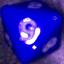
\includegraphics[width=\linewidth]{chapters/04-czytanie/figures/blask_raw}
        \caption{Odblask na przeskalowanym zdjęciu.}
        \label{fig:blaskraw}
    \end{subfigure}
    \hfill
    \begin{subfigure}[t]{0.45\linewidth}
        \centering
        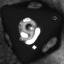
\includegraphics[width=\linewidth]{chapters/04-czytanie/figures/blask_proc}
        \caption{Odblask po zmianie na skalę szarości.}
        \label{fig:blaskproc}
    \end{subfigure}
    \caption{Porównanie przetwarzania odblasku: część a) i b).}
    \label{fig:blaskcombined}
\end{figure}


Inną trudnością, która objawiała się w początkowych fazach pracy były zupełnie czarne obrazy,
w wyniku problemu z działaniem diod, jednak problem okazał się być spowodowany przez hardware --
pomogło lepsze zaizolowanie przewodów kamery i diod.

Mimo zażegnania problemu w taki sposób, zapewniono również obsługę wyjątku,
który nadarzy się gdy do preprocessu trafi zupełnie czarne zdjęcie -- taki przypadek jest pomijany.
W przypadku trzech takich nieprawidłowych zdjęć pod rząd generator przerywa pracę zgłaszając błąd.
W podobny sposób postarano się o wykrycie zacięcia się śmigła,
co znaczy że preprocess dostaje cały czas takie same zdjęcie do obróbki.
Tu również zadbano o to, by to wykrywać, jednak w związku z ryzykiem losowego podobieństwa kilku rzutów następujących po sobie,
a więc ryzyka nieprawidłowego wykrycia błędu, % nie wiem jak to nazwaććććć
przerwanie pracy następuje dopiero po 13 identycznych odczytach z rzędu.
Statystyczna szansa na takie zdarzenie przy prawidłowej pracy maszyny wynosi
$\frac{1}{8^{12}} \approx 1{,}455 \times 10^{-11}$
%tak, zmieniliśmy na 13 żeby tego nie przeliczać znowu.
%a właściwie nie zmieniliśmy, bo w kodzie już było implementowane 13, bo tam zrobiłem ten sam off-by-one error, więc wszystko się zgadzało poza opisem
%PS: Na probabilistyce jeszcze pamiętałem o takich rzeczach! Przepraszam!
%%PPS: Mnie przepuścił Pana kolega, który potem niechcący zabrał mi miejsce na angielskim...


Kolejną, znacznie częściej spotykaną trudnością w obecnej architekturze urządzenia są niejednoznaczne wyniki,
a więc moment gdy kość zatrzyma się w pozycji w której widać więcej niż jedną ściankę.
Najczęściej jest to spowodowane tym, że kostka zatrzymała się na śmigle napędowym,
przez co wynik może być niejednoznaczny, co pokazano na rysunkach~\ref{fig:smiglocombined}.
% TODO check nazwy śmigło!

\begin{figure}[h]
    \centering
    \begin{subfigure}[t]{0.45\linewidth}
        \centering
        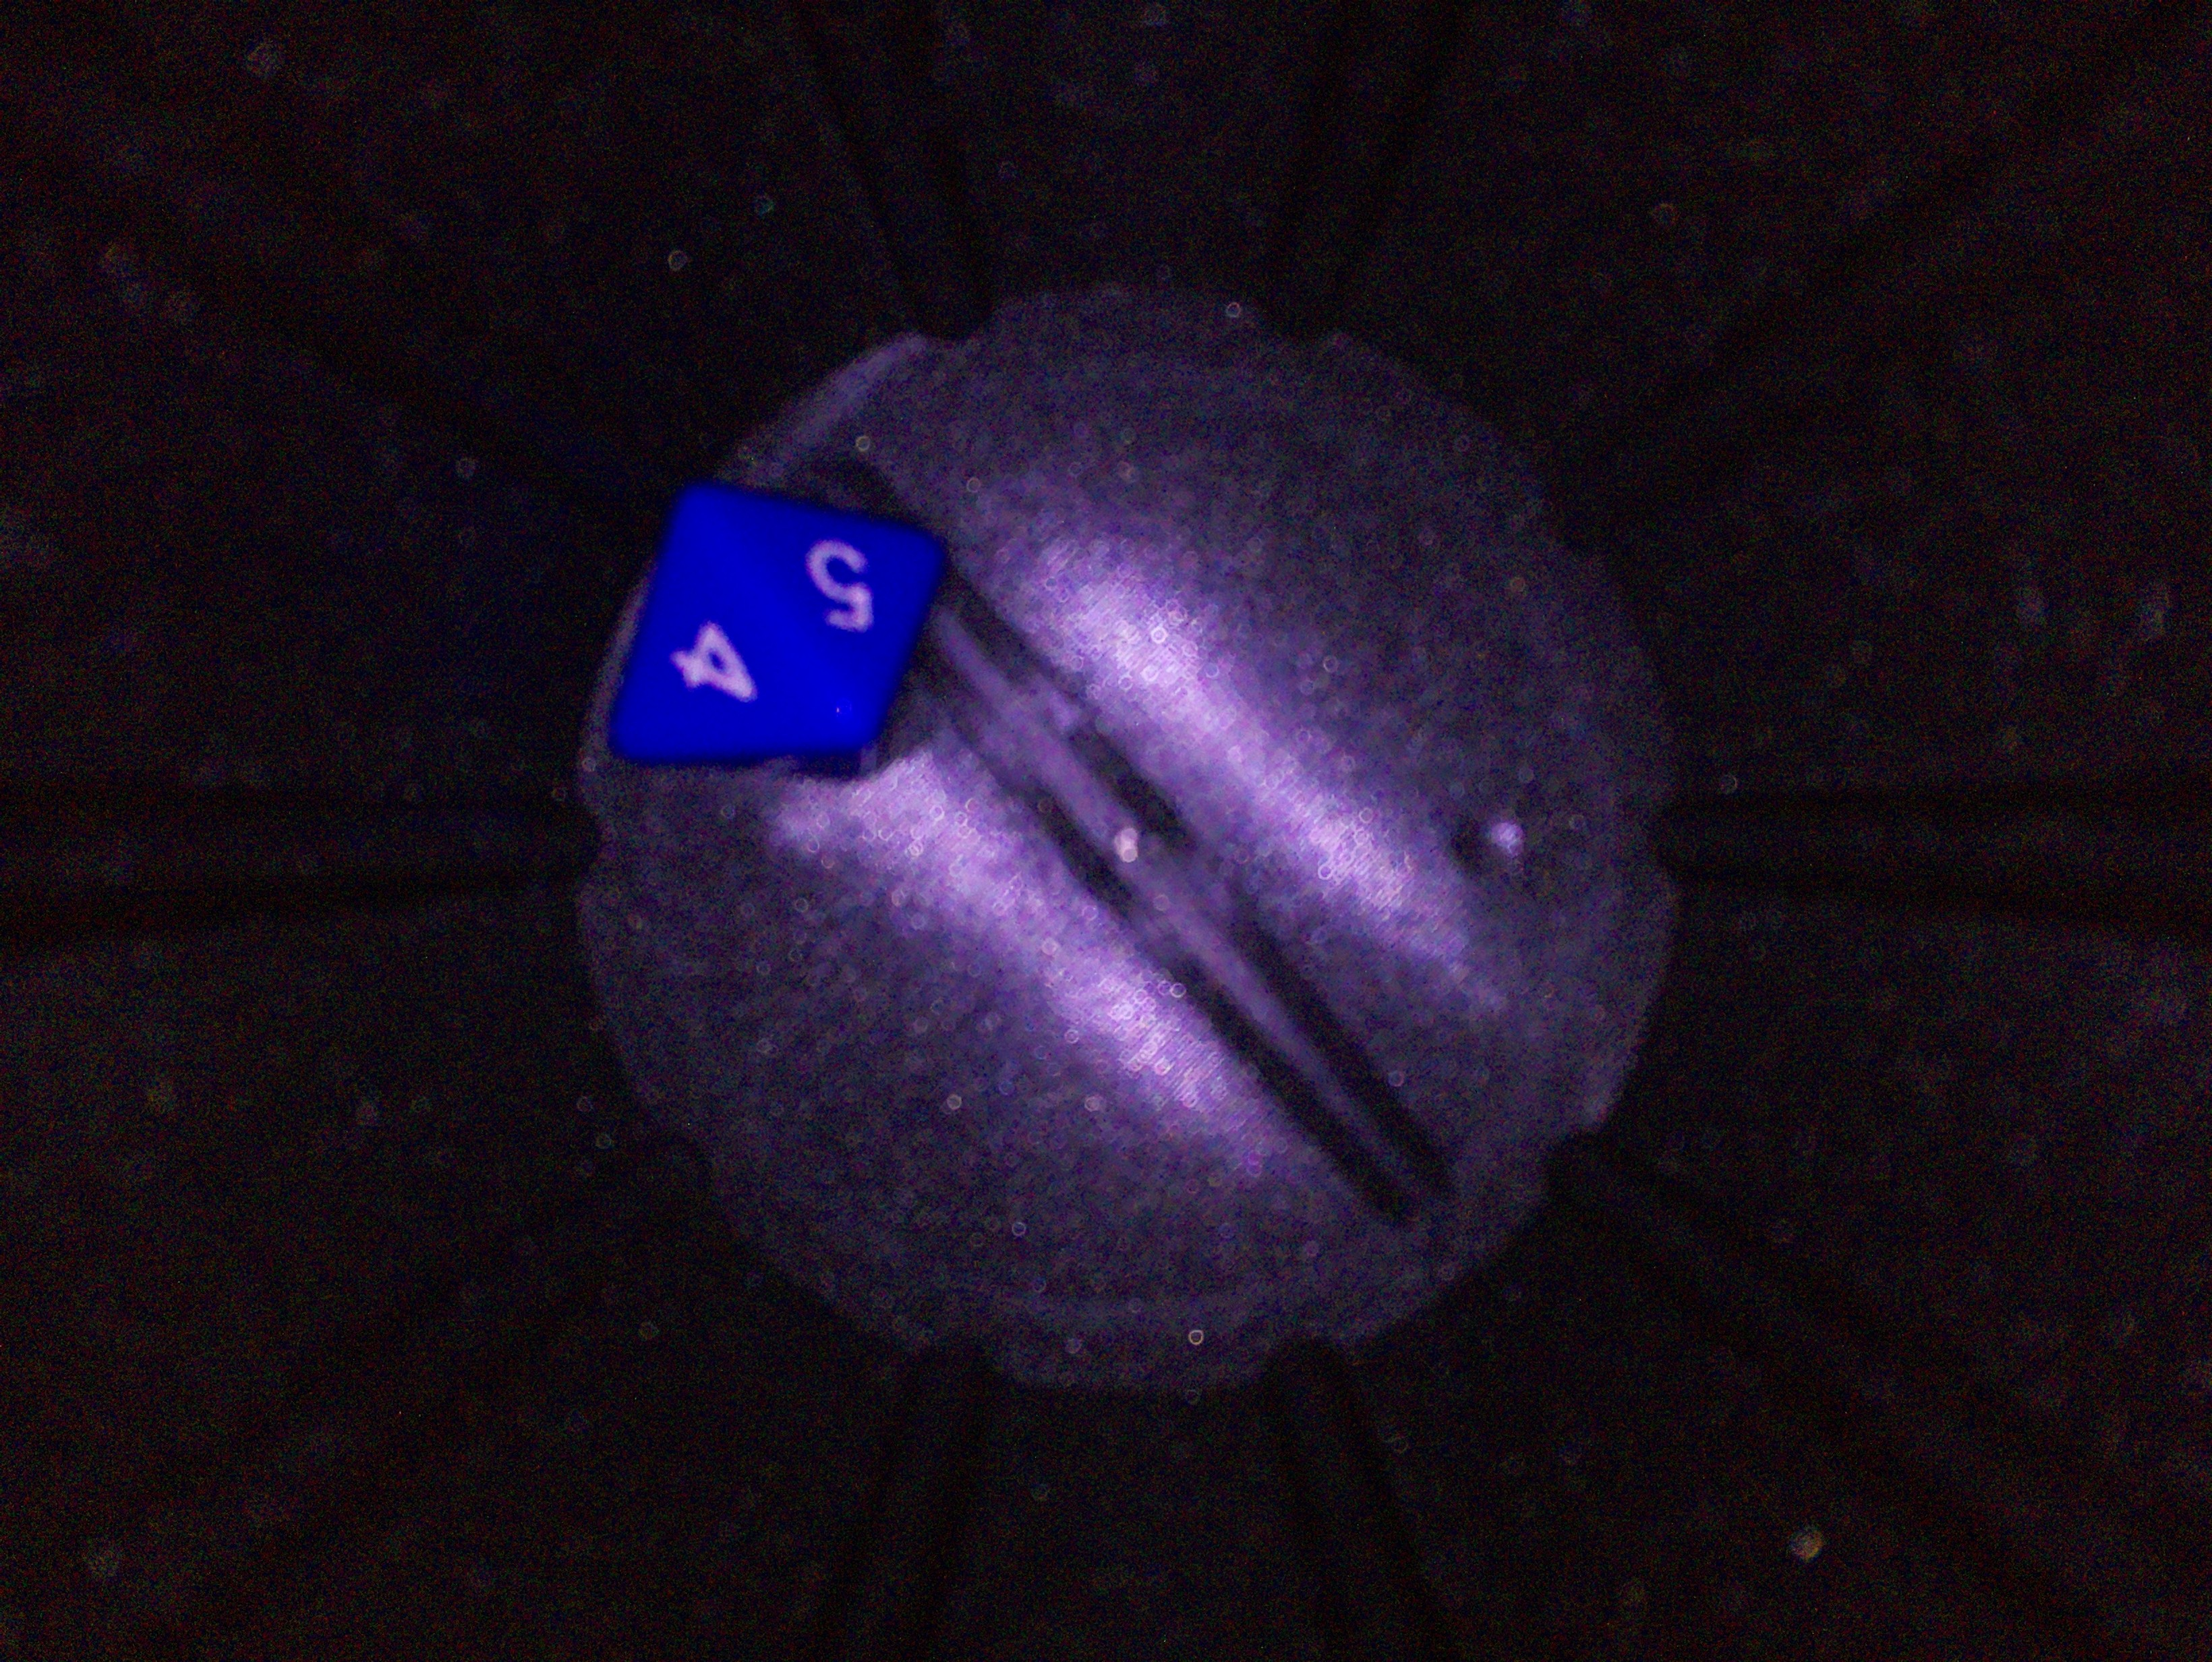
\includegraphics[width=\linewidth]{chapters/04-czytanie/figures/niepewne}
        \caption{Kość zatrzymana na śmigle (ujęcie 1).}
        \label{fig:niepewne}
    \end{subfigure}
    \hfill
    \begin{subfigure}[t]{0.45\linewidth}
        \centering
        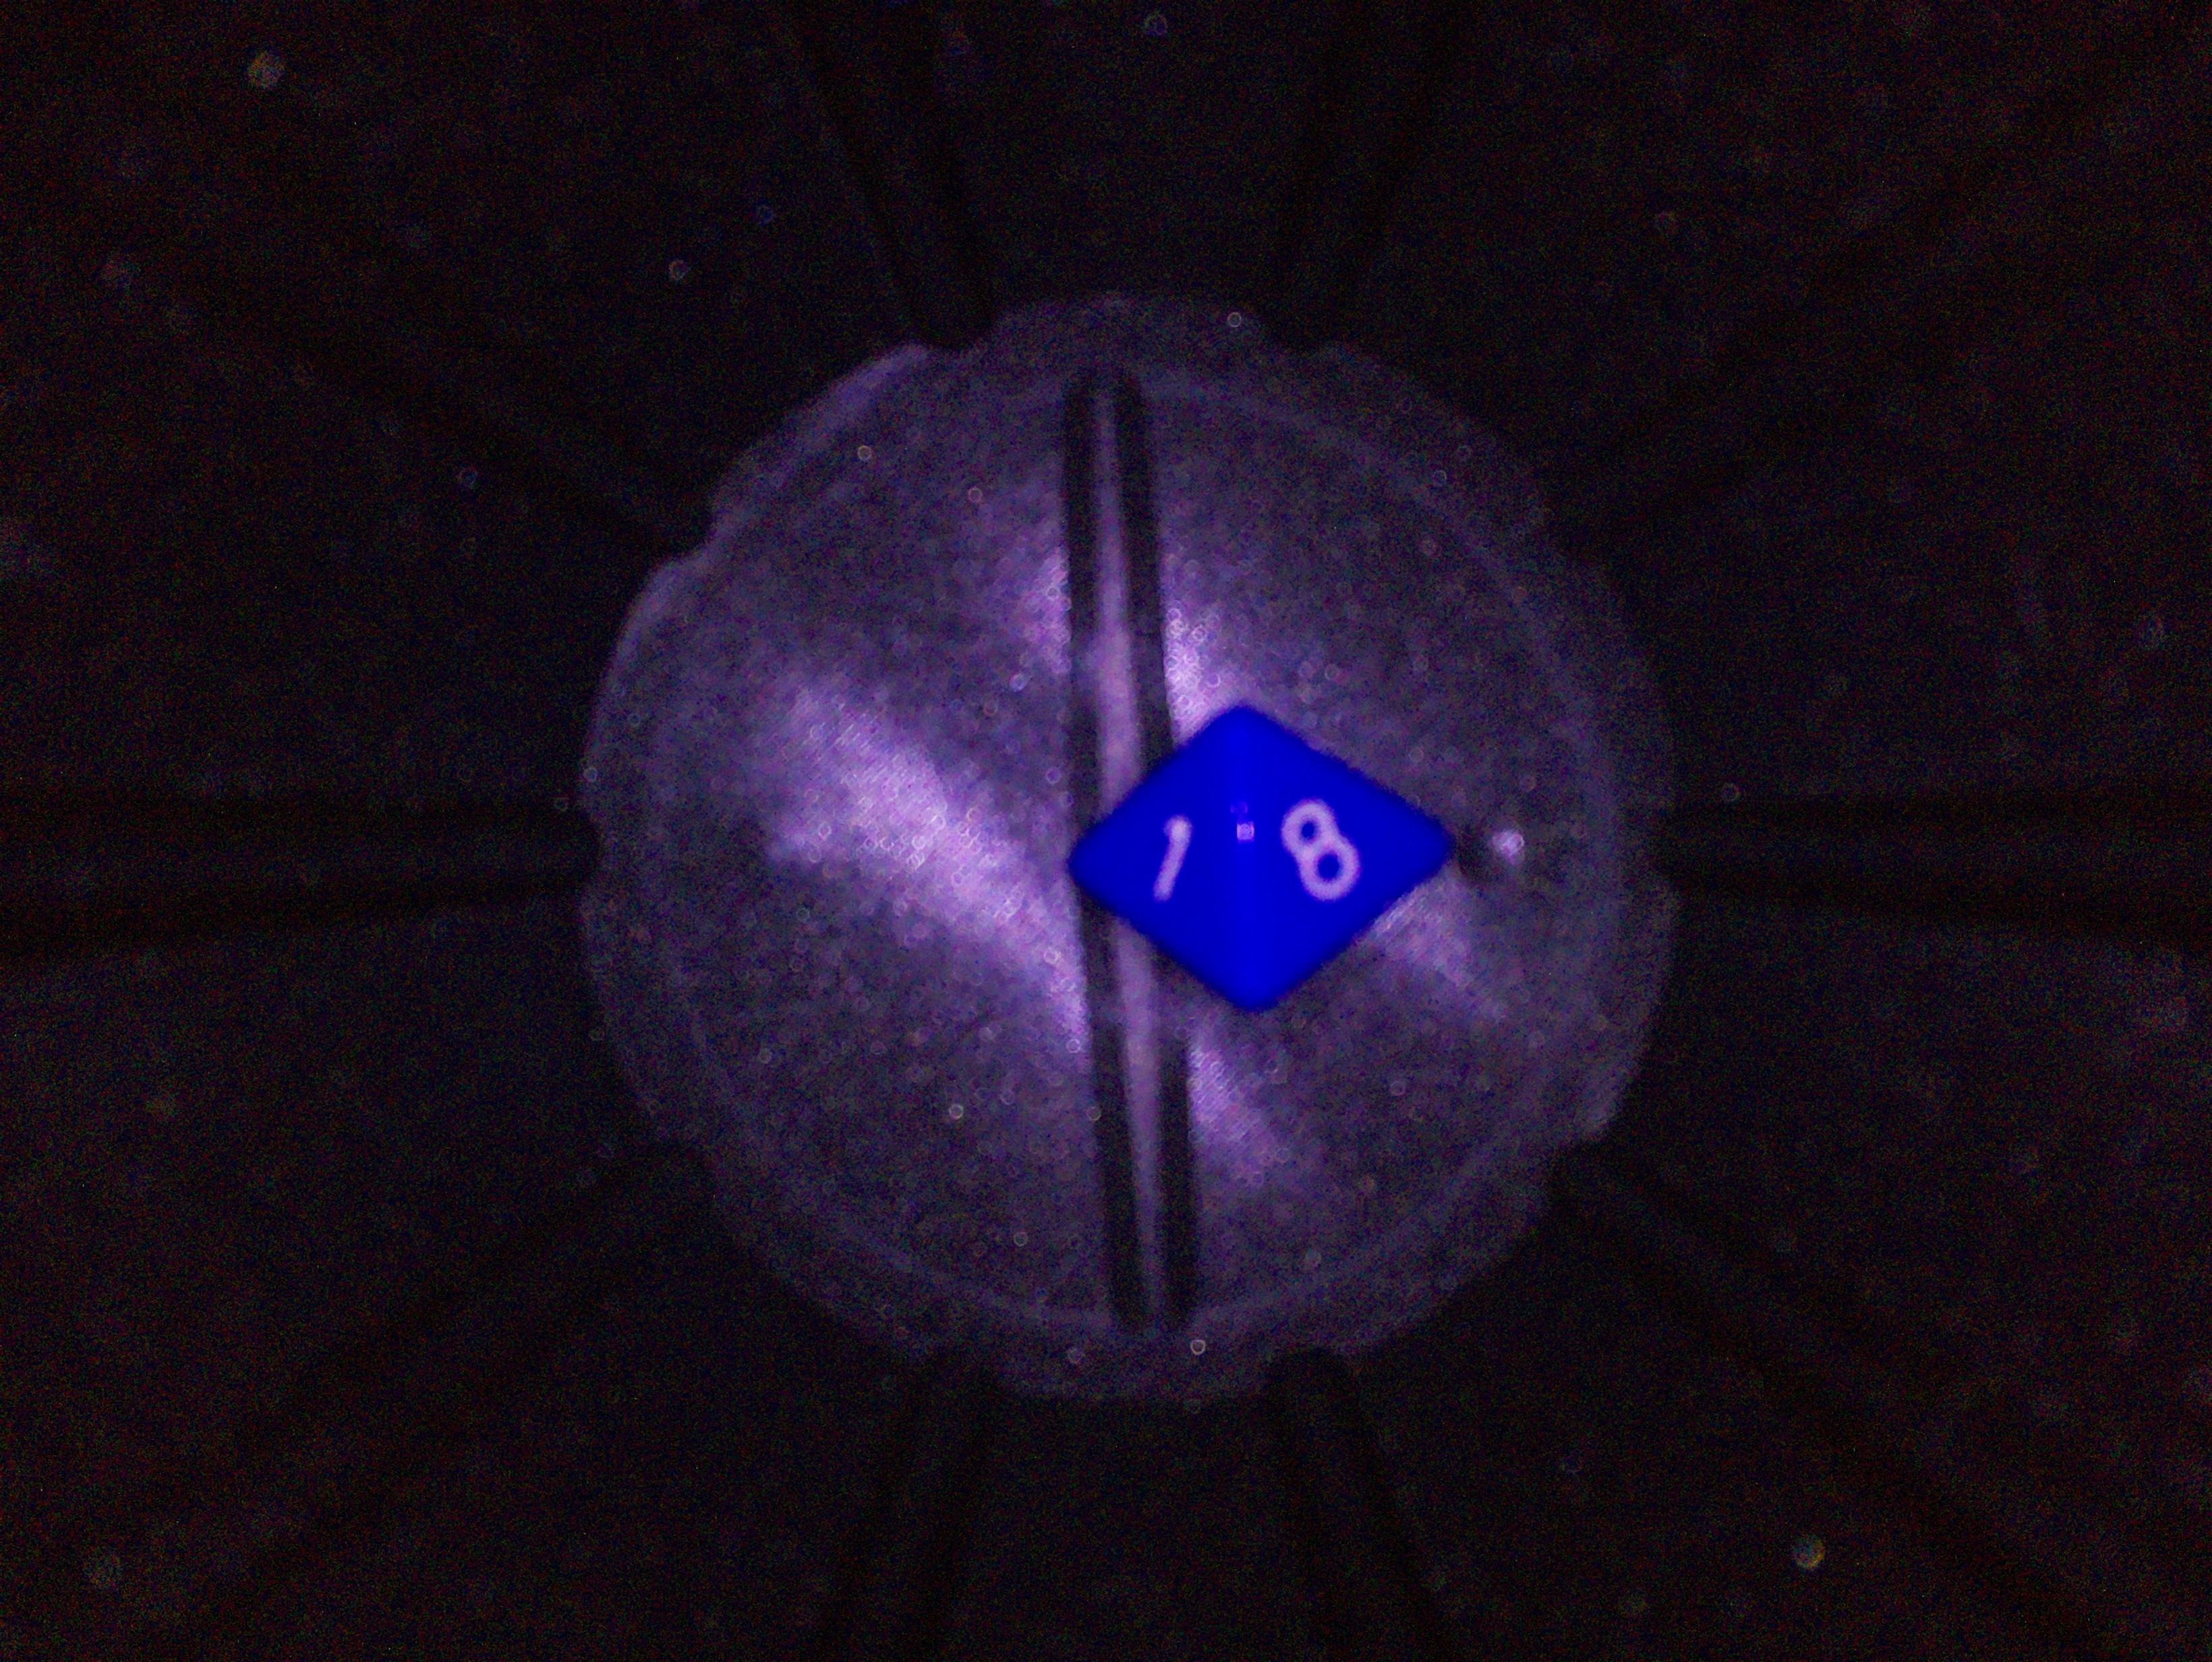
\includegraphics[width=\linewidth]{chapters/04-czytanie/figures/smiglo}
        \caption{Kość zatrzymana na śmigle (ujęcie 2).}
        \label{fig:smiglo}
    \end{subfigure}
    \caption{Porównanie dwóch ujęć kości zatrzymanej na śmigle.}
    \label{fig:smiglocombined}
\end{figure}


Rozwiązaniem tego problemu jest model dokonujący klasyfikacji wyniku rzutu, który siłą rzeczy odczytuje ze zdjęcia tylko jeden wynik i wybiera ten,
który jest bardziej widoczny, ponieważ podczas uczenia model miał do czynienia z takimi niejednoznacznymi sytuacjami,
które byliśmy w stanie ręcznie oznaczyć właśnie na potrzeby treningu modelu.

Zdarzają się oczywiście rzadkie przypadki, w których kość wyląduje równo na śmigle, tak że wynik jest idealnie czytelny,
tak jakby wylądowała normalnie na podstawce kubka, ale wtedy problem z lądowaniem na śmigle nie istnieje,
gdyż nie przeszkadza to w tym że kość i tak zostanie podbita przy następnym obrocie śmigła.


Ostatnim rodzajem problemu jaki został napotkany był przypadek w którym kostka nie skończyła jeszcze swojej fazy lotu,
lub wpadła w bardzo długie wirowanie -- efektywnie uniemożliwiając odczytanie wyniku.

\begin{figure}[h]
    \centering
    \begin{subfigure}[t]{0.45\linewidth}
        \centering
        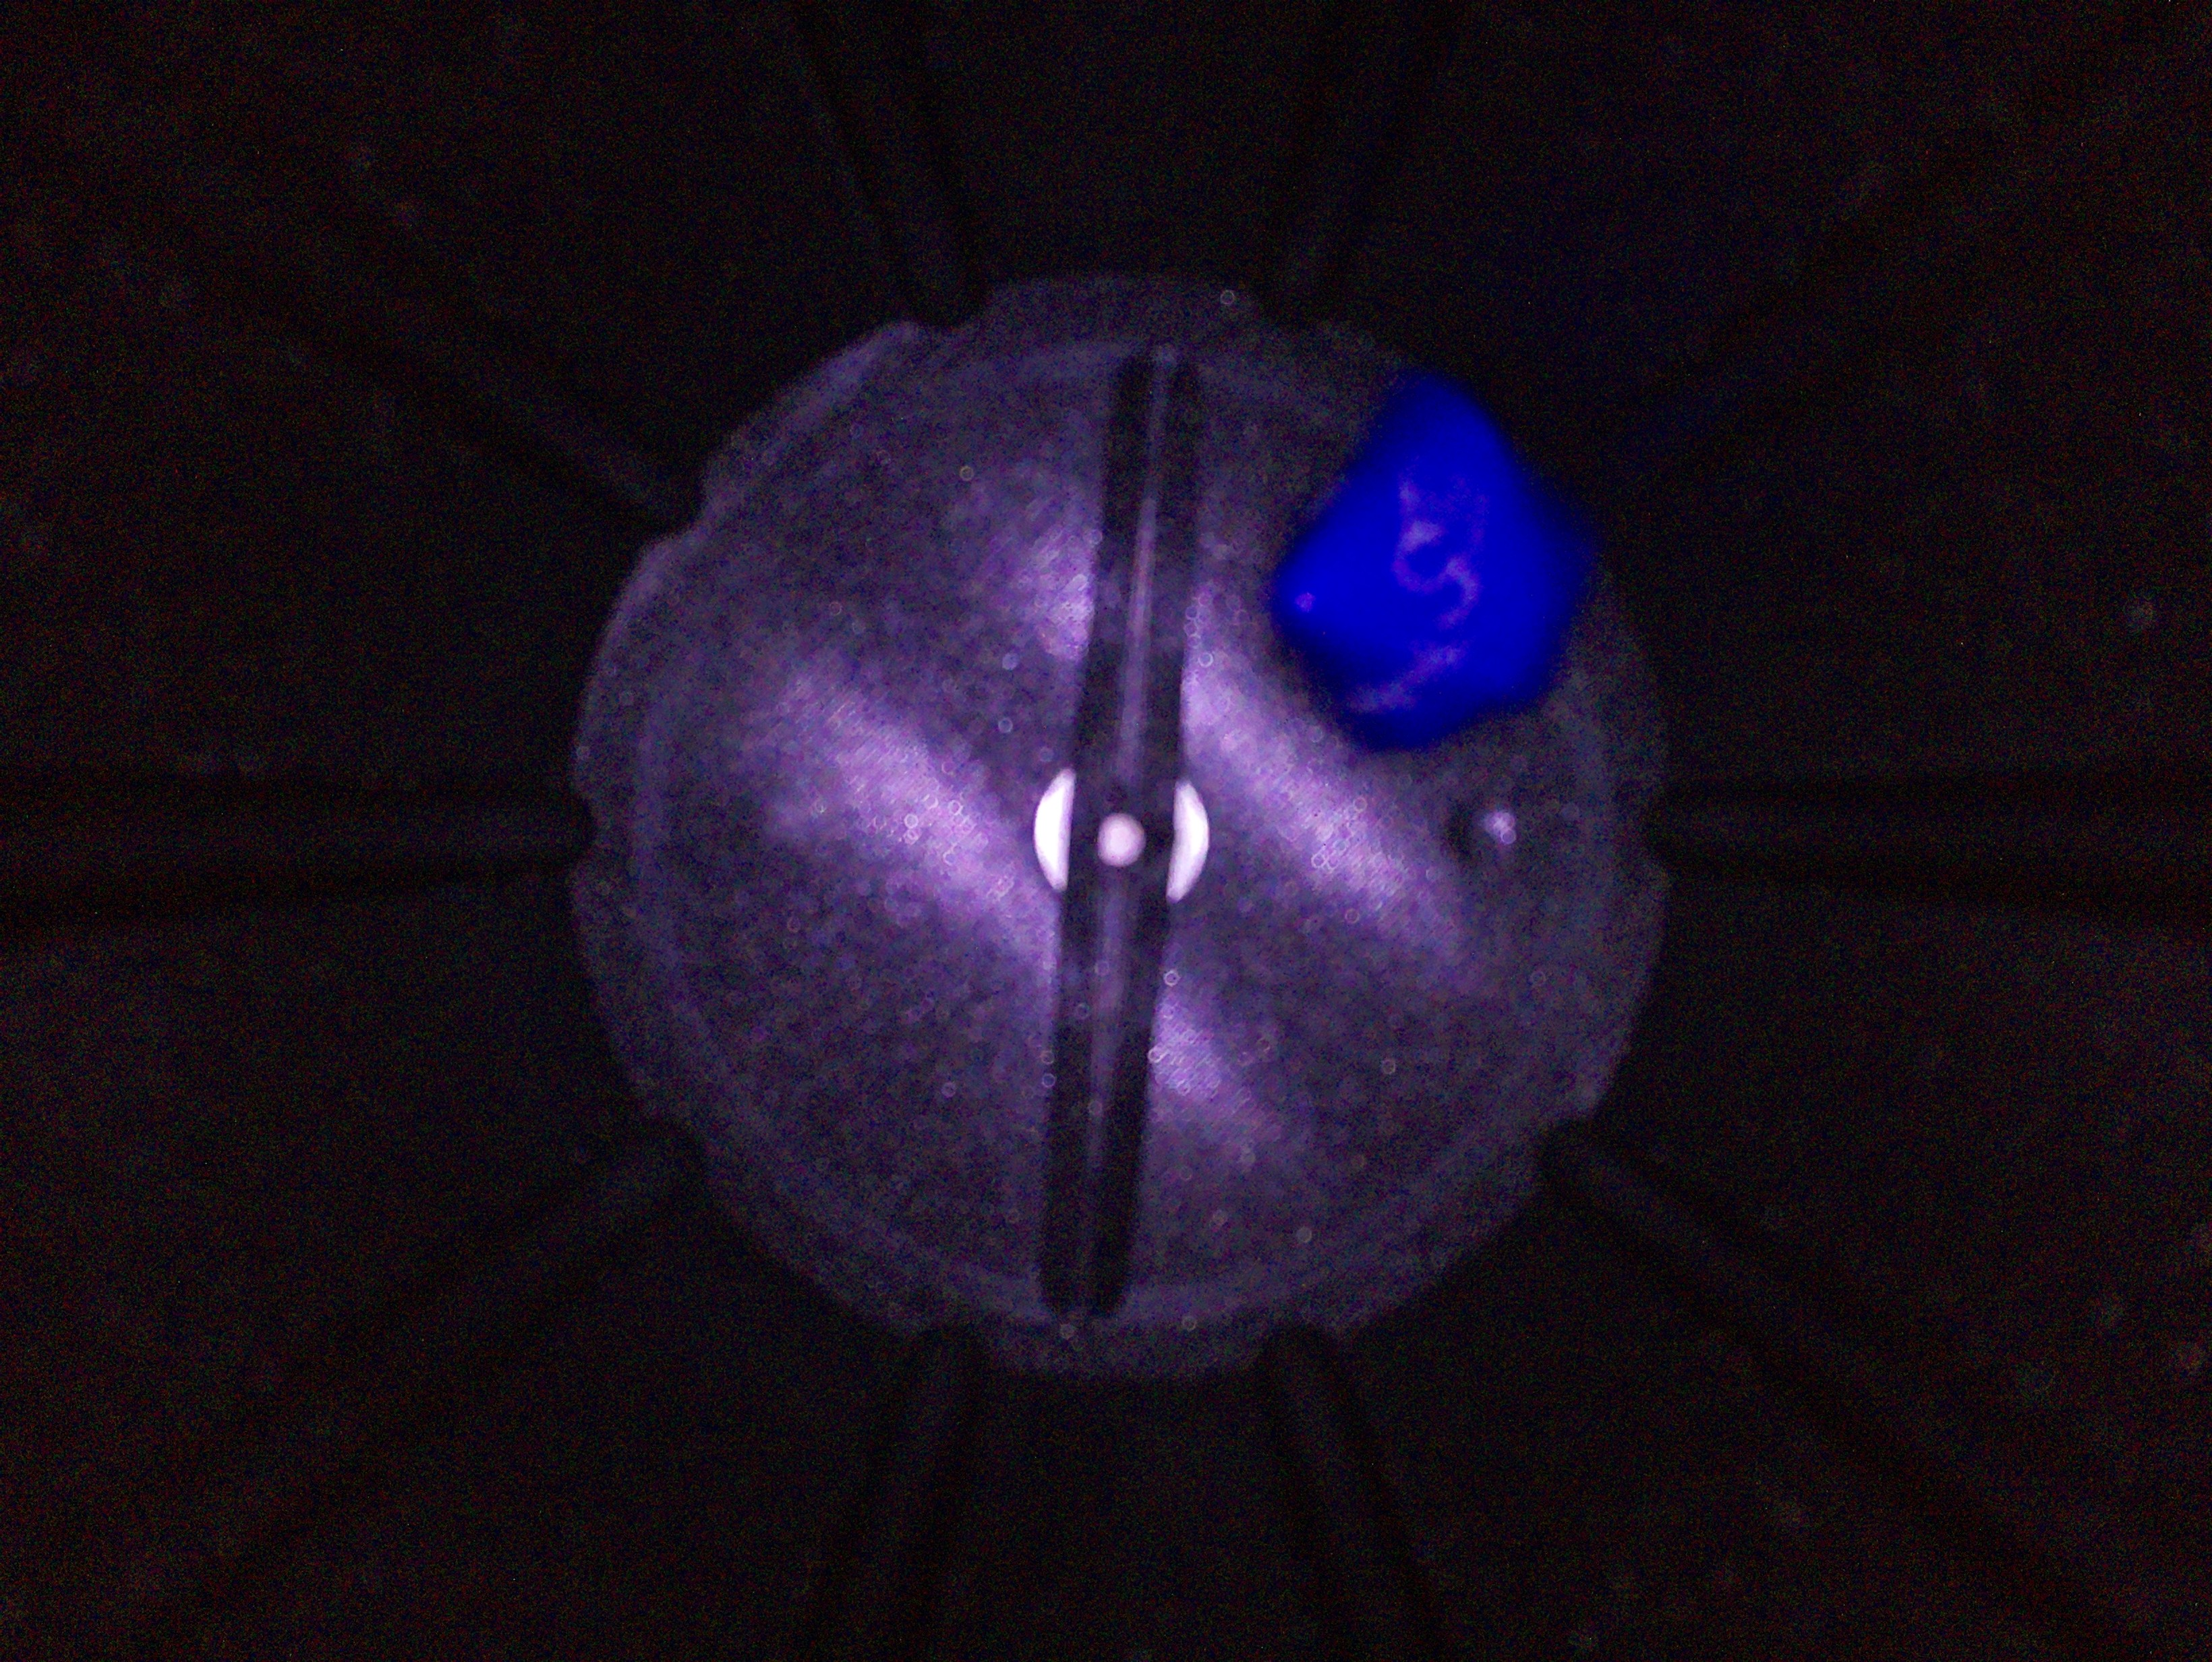
\includegraphics[width=\linewidth]{chapters/04-czytanie/figures/wir}
        \caption{Wirująca kość.}
        \label{fig:wir}
    \end{subfigure}
    \hfill
    \begin{subfigure}[t]{0.45\linewidth}
        \centering
        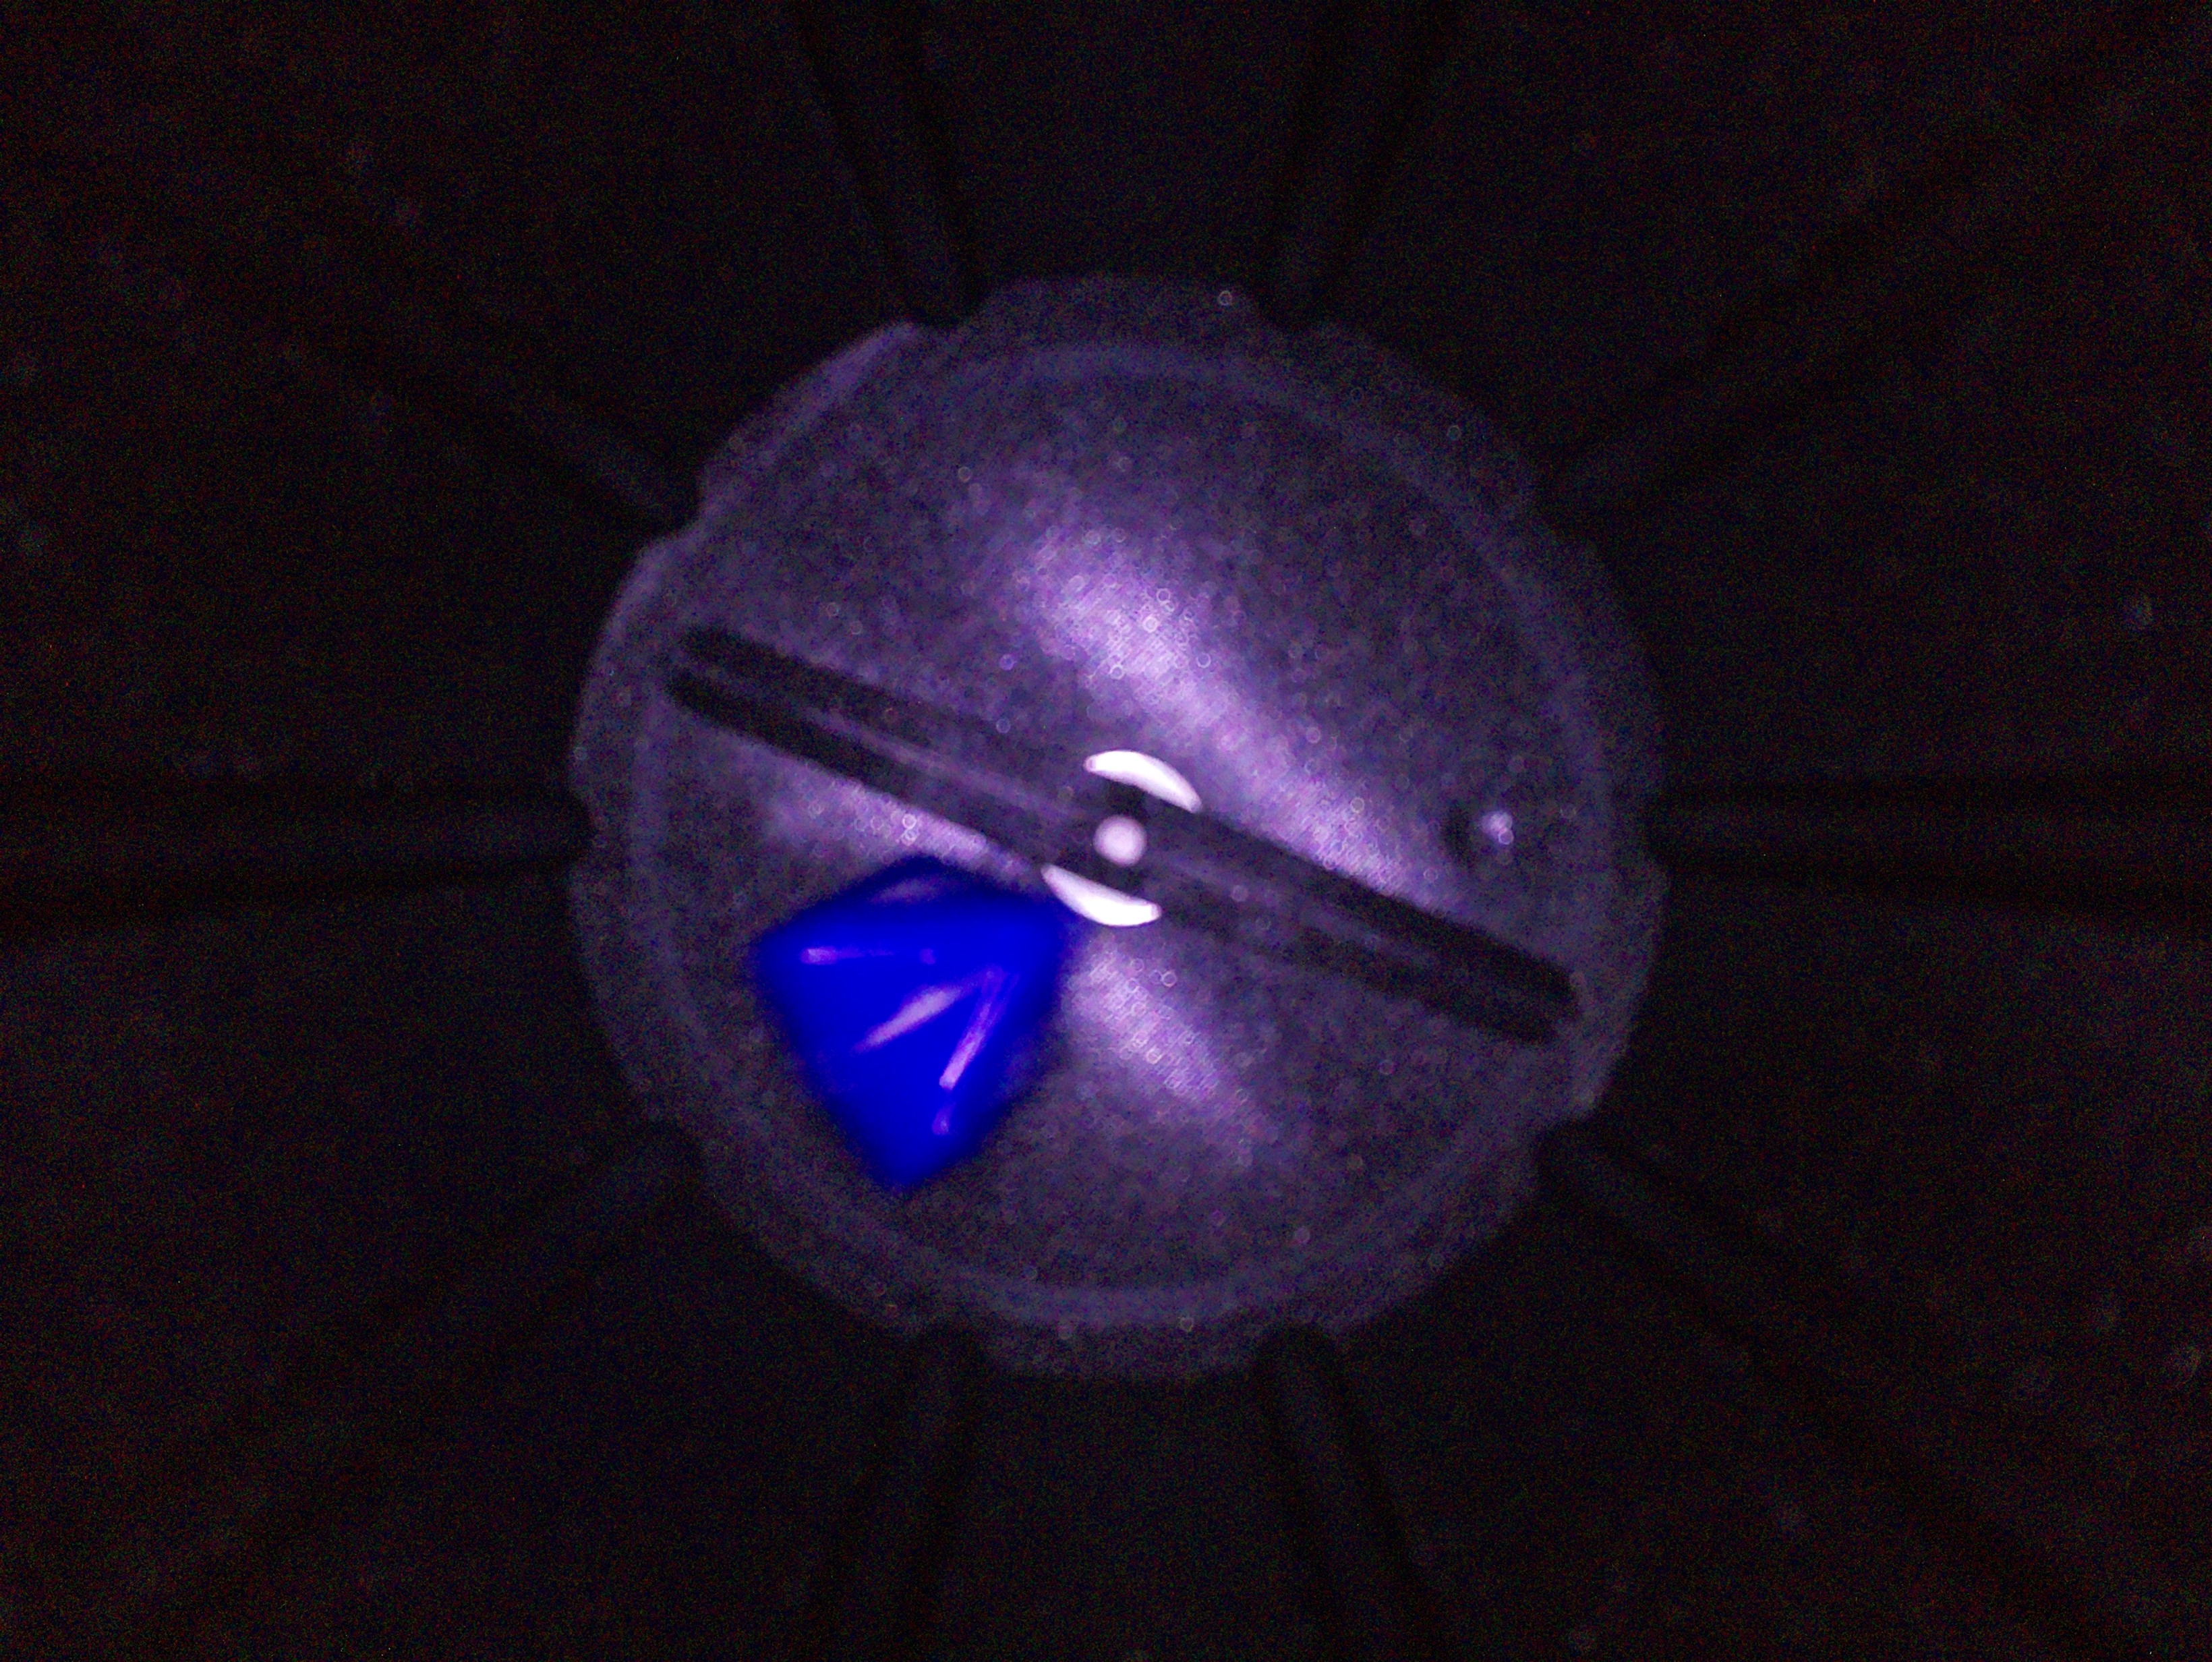
\includegraphics[width=\linewidth]{chapters/04-czytanie/figures/wir2}
        \caption{Kość w ruchu.}
        \label{fig:wir2}
    \end{subfigure}
    \caption{Nieczytelne ujęcia wynikające z dłuższego niż przewidywany ruchu kości}
    \label{fig:wircombined}
\end{figure}


Rozwiązaniem większości wypadków w których zachodziła ta sytuacja okazało się spowolnienie działania maszyny.
Obecnie, oczekiwaniem aż kość zatrzyma się w miejscu steruje parametr czasowy, przyjmujący wartość jednej sekundy od zakończenia pracy śmigła.
Jest to wystarczające rozwiązanie, gdyż obecnie sytuacje niepewne z tego powodu zdarzają się bardzo rzadko (około 1 raz na 5000 rzutów).

Istnieje możliwość udoskonalenia tego rozwiązania, poprzez stosowanie detekcji ruchu kości,
jednak to rozwiązanie najpewniej okazałoby się bardziej kosztowne czasowo niż to proste czekanie stosowane obecnie.


\subsection{Podsumowanie}\label{subsec:podsumowanie}

Przedstawiony algorytm przetwarzania wstępnego pozwala na skuteczne przygotowanie danych wejściowych dla modelu sztucznej inteligencji.
Automatyzuje proces identyfikacji i kadrowania obiektów zainteresowania w obrazach, co znacząco poprawia jakość danych.
Rozwiązanie zostało zaprojektowane z myślą o łatwej adaptacji do innych zastosowań wymagających podobnego przetwarzania obrazów,
dla przykładu przypadku zmiany kości w maszynie na inną, lub z inną liczbą ścianek.

